\chapter{Аналитическая часть}

В данном разделе представлено теоретическое описание алгоритма гномьей сортировки, сортировки бусинами и подсчетом.

\section{Алгоритм сортировки бусинами}

Рассмотрим массив $arr$ из $n$ положительных целых чисел, которые нужно отсортировать, и предположим, что максимальный элемент массива arr --- число $m$. Тогда каркас с бусинами должен иметь не менее $m$ стержней и $n$ уровней (см. рис. \ref{img:bead_sort_fig} \cite{bead_sort}). 

\begin{figure}[H]
	\begin{center}
		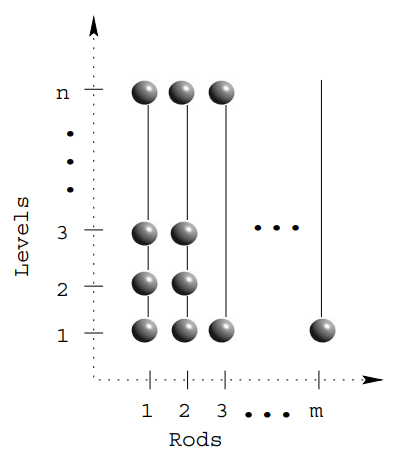
\includegraphics[scale=0.7]{img/bead_sort_fig.png}
	\end{center}
	\captionsetup{justification=centering}
	\caption{Каркас с бусинами}
	\label{img:bead_sort_fig}
\end{figure}

Идея алгоритма сортировки бусинами заключается в том, чтобы для каждого элемента $x$ массива $arr$ надеть на каждый стержень по бусине, начиная от $1$-го стержня до $x$-го стержня. Таким образом, бусины, представленные на каждом уровне, начиная с $n$-го уровня до $1$-го уровня представляют массив $arr$ в порядке возрастания \cite{bead_sort}.

\section{Алгоритм сортировки подсчетом}

Сортировка подсчетом является сортировкой без сравнений (см. пример на рис.\ref{img:counting_sort_fig}).
Рассмотрим массив $A[0..n-1]$, содержащий
неотрицательные целые числа меньшие $k$.
Алгоритм сортировки подсчетом состоит из следующих шагов:
\begin{itemize}
	\item заведем массив $C[0..k-1]$;
	\item посчитаем в $C[i]$ количество вхождений элемента $i$ в массиве $A$;
	\item запишем в массив $A$ все элементы $C$ по $C[i]$ раз.
\end{itemize}

\begin{figure}[H]
	\begin{center}
		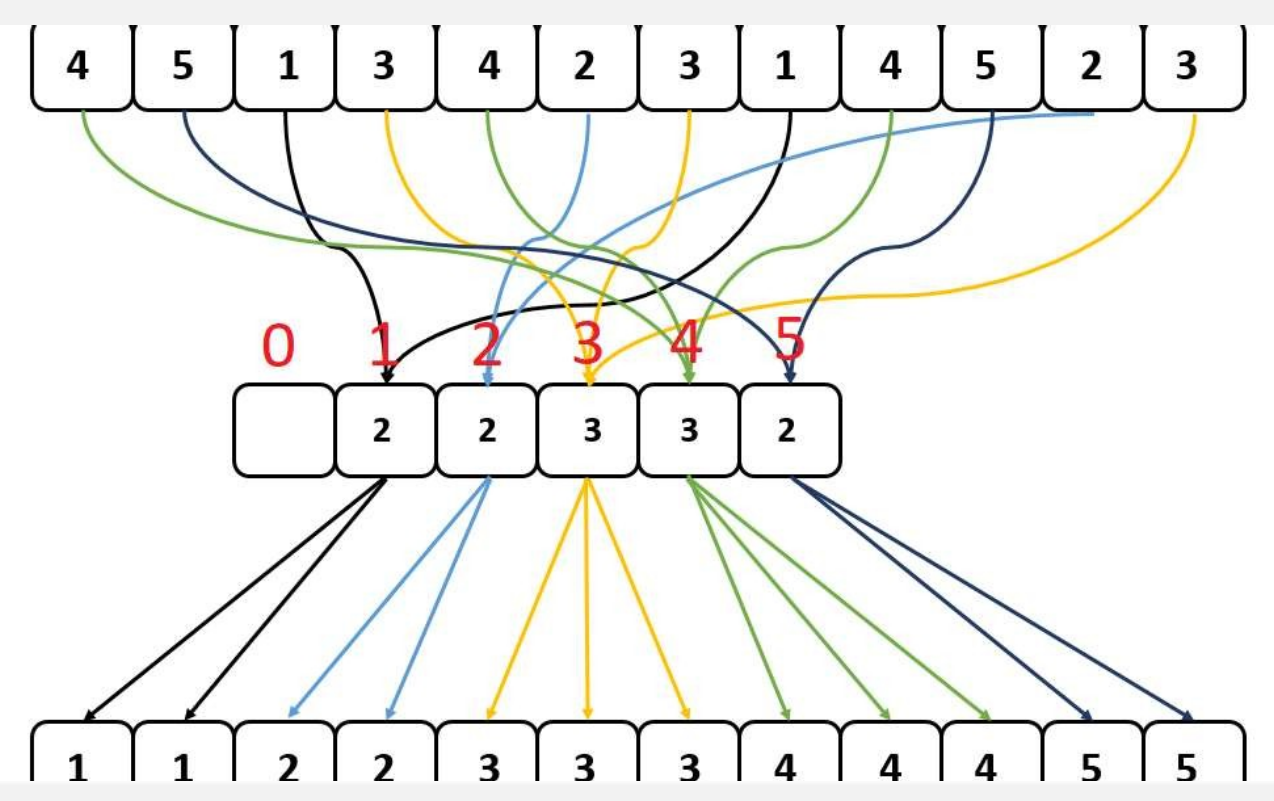
\includegraphics[scale=0.4]{img/counting_sort_fig.png}
	\end{center}
	\captionsetup{justification=centering}
	\caption{Сортировка подсчетом}
	\label{img:counting_sort_fig}
\end{figure}


\section{Алгоритм гномьей сортировки}

Для начала сравнения указатель ставится на второй элемент
массива. После этого происходит cравнение текущего и предыдущего элементов. Если порядок соблюден --- происходит переход к следующему элементу, если нет, то элементы меняются местами и указатель в цикле переходит к предыдущему элементу. Цикл сортировки заканчивается в тот момент, когда номер указателя становится равным длине массива \cite{gnome_sort}.


\section*{Вывод}

В данном разделе были описаны основные положения алгоритмов сортировки: бусинами, подсчетом и гномьей сортировки.